 我々はまず、前立腺の病理画像をGP(Gleason pattern)に応じて正常腺管、GP3、GP4、GP5のセマンティックセグメンテーション(Semantic segmentation、画像を意味に基づいてピクセル単位で区分する手法)を行うU-Netモデルを作成した。そのモデルは、当教室で診断された前立腺全摘出標本と独自に作成GPラベルによって訓練されている。\par
\vspace{0.5zh}
 また、HTTP経由で画像が送信された際に、その画像をDLによって解析し、その結果を配信するサーバーアプリケーションと、USBカメラから入力される映像をHTTP経由で送信するクライアントアプリケーションを作成した。サーバーアプリケーションはDLの動作するコンピュータに、クライアントアプリケーションは顕微鏡カメラとUSB接続したRaspberry Pi 4 Model Bにそれぞれ導入した。\par

\begin{figure}
\begin{center}
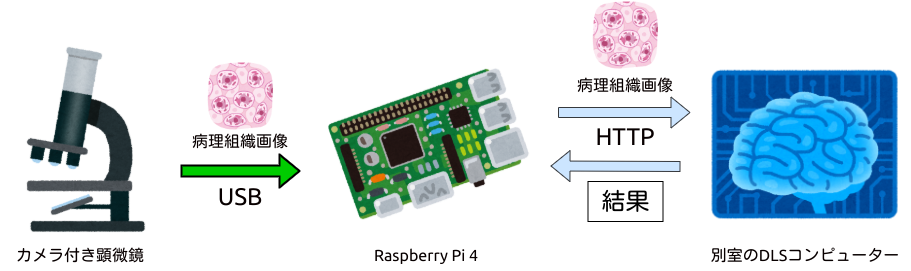
\includegraphics[width=\columnwidth]{fig1.png}
\small [1]アプリケーション構成図
\end{center}
\end{figure}
\vspace{1zh}
